%----------------------------------------------------------------------------------------

\documentclass[a4paper,10pt]{article} % Uses article class in A4 format

%----------------------------------------------------------------------------------------
%	FORMATTING
%----------------------------------------------------------------------------------------

\setlength{\parskip}{0pt}
\setlength{\parindent}{0pt}
\setlength{\voffset}{-15pt}

%----------------------------------------------------------------------------------------
%	PACKAGES AND OTHER DOCUMENT CONFIGURATIONS
%----------------------------------------------------------------------------------------

\usepackage[a4paper, margin=2.5cm]{geometry} % Sets margin to 2.5cm for A4 Paper
\usepackage[onehalfspacing]{setspace} % Sets Spacing to 1.5

\usepackage[T1]{fontenc} % Use European encoding
\usepackage[utf8]{inputenc} % Use UTF-8 encoding
\usepackage{charter} % Use the Charter font
\usepackage{microtype} % Slightly tweak font spacing for aesthetics

\usepackage[english]{babel} % Language hyphenation and typographical rules

\usepackage{amsthm, amsmath, amssymb} % Mathematical typesetting
\usepackage{marvosym, wasysym} % More symbols
\usepackage{float} % Improved interface for floating objects
\usepackage[final, colorlinks = true, 
            linkcolor = black, 
            citecolor = black,
            urlcolor = black]{hyperref} % For hyperlinks in the PDF
\usepackage{graphicx, multicol} % Enhanced support for graphics
\usepackage{xcolor} % Driver-independent color extensions
\usepackage{rotating} % Rotation tools
\usepackage{listings, style/lstlisting} % Environment for non-formatted code, !uses style file!
\usepackage{pseudocode} % Environment for specifying algorithms in a natural way
\usepackage{style/avm} % Environment for f-structures, !uses style file!
\usepackage{booktabs} % Enhances quality of tables

\usepackage{tikz-qtree} % Easy tree drawing tool
\tikzset{every tree node/.style={align=center,anchor=north},
         level distance=2cm} % Configuration for q-trees
\usepackage{style/btree} % Configuration for b-trees and b+-trees, !uses style file!

\usepackage{titlesec} % Allows customization of titles
\renewcommand\thesection{\arabic{section}.} % Arabic numerals for the sections
\titleformat{\section}{\large}{\thesection}{1em}{}
\renewcommand\thesubsection{\alph{subsection})} % Alphabetic numerals for subsections
\titleformat{\subsection}{\large}{\thesubsection}{1em}{}
\renewcommand\thesubsubsection{\roman{subsubsection}.} % Roman numbering for subsubsections
\titleformat{\subsubsection}{\large}{\thesubsubsection}{1em}{}

\usepackage[all]{nowidow} % Removes widows

\usepackage[backend=biber,style=numeric,
            sorting=nyt, natbib=true]{biblatex} % Complete reimplementation of bibliographic facilities
\addbibresource{main.bib}
\usepackage{csquotes} % Context sensitive quotation facilities

\usepackage[yyyymmdd]{datetime} % Uses YEAR-MONTH-DAY format for dates
\renewcommand{\dateseparator}{-} % Sets dateseparator to '-'

\usepackage{fancyhdr} % Headers and footers
\pagestyle{fancy} % All pages have headers and footers
\fancyhead{}\renewcommand{\headrulewidth}{0pt} % Blank out the default header
\fancyfoot[L]{\textsc{Robin Worreby}} % Custom footer text
\fancyfoot[C]{} % Custom footer text
\fancyfoot[R]{\thepage} % Custom footer text

\newcommand{\note}[1]{\marginpar{\scriptsize \textcolor{red}{#1}}} % Enables comments in red on margin
\usepackage[shortlabels]{enumitem}
\usepackage{minted}
\usemintedstyle{friendly}
\usepackage[bf]{caption}
%----------------------------------------------------------------------------------------

\begin{document}

%----------------------------------------------------------------------------------------
%	TITLE SECTION
%----------------------------------------------------------------------------------------

\title{template_assignment} % Article title
\fancyhead[C]{}
\begin{minipage}{0.295\textwidth} % Left side of title section
\raggedright
HPCSE1\\ % Your lecture or course
\footnotesize % Authors text size
%\hfill\\ % Uncomment if right minipage has more lines
Robin Worreby, 16-921-298 % Your name, your matriculation number
\medskip\hrule
\end{minipage}
\begin{minipage}{0.4\textwidth} % Center of title section
\centering 
\large % Title text size
Exercise 02\\ % Assignment title and number
\normalsize % Subtitle text size
OpenMP\\ % Assignment subtitle
\end{minipage}
\begin{minipage}{0.295\textwidth} % Right side of title section
\raggedleft
\today\\ % Date
\footnotesize % Email text size
%\hfill\\ % Uncomment if left minipage has more lines
rworreby@student.ethz.ch% Your email
\medskip\hrule
\end{minipage}

%----------------------------------------------------------------------------------------
%	ARTICLE CONTENTS
%----------------------------------------------------------------------------------------

\setcounter{section}{0}

\section{Parallel Monte Carlo using OpenMP}

\begin{enumerate}[b)]
\setcounter{enumi}{0}
\item

We benchmark the four implementations on our local computer and on the Euler cluster with up to 24 threads on each. We repeat the measurements once for the compiler flag $-O0$ and once for $-O3$ on both systems. The results can be seen in Figures \ref{fig:local_O0} to \ref{fig:euler_O3}. The behaviour on both our local machine and on the Euler cluster are very similar and look qualitatively roughly the same. Two distinct things to notice are that in the case of $-O0$ we can observe false sharing as the unpadded array implementation in both cases performs significantly worse than the other implementations. On the local machine the unpadded array implementation even performs worse than the serial implementation, up to 6 threads. Another thing to notice is that the implementation without array is performing better than the other implementations on our local machine, but no distinct improvement is noticeable on the Euler cluster. 

\begin{figure}[h]
  \centering
  \begin{minipage}[t]{0.45\textwidth}
    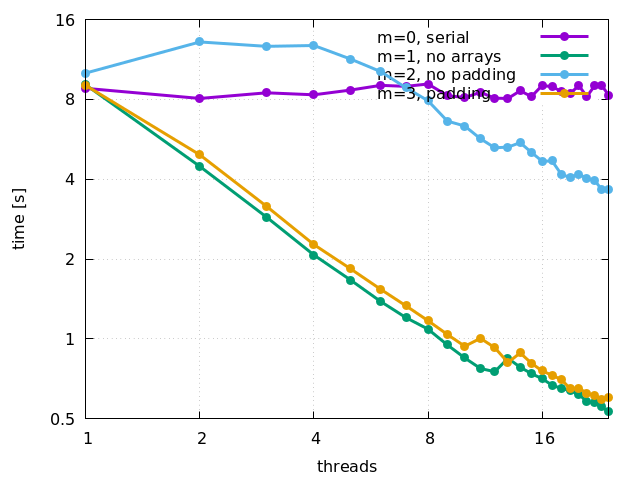
\includegraphics[width=\textwidth]{plots/scaling_local_O0.png}
    \caption{Scaling behavior on local computer for 4 different implementations. Parameter $-O0$.}
    \label{fig:local_O0}
  \end{minipage}
  \hfill
  \begin{minipage}[t]{0.45\textwidth}
    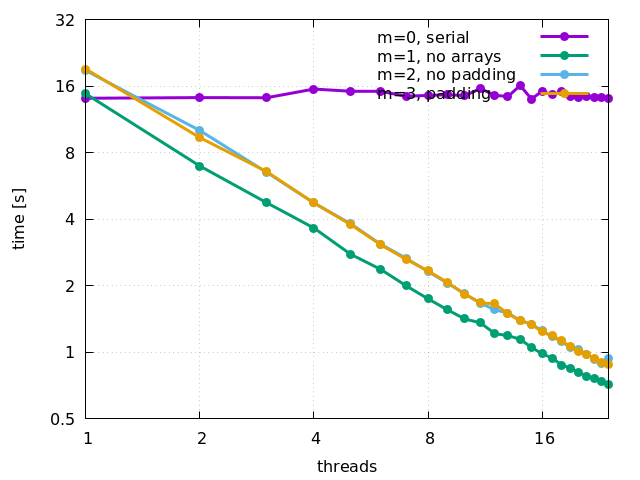
\includegraphics[width=1\textwidth]{plots/scaling_local_O3.png}
    \caption{Scaling behavior on local computer for 4 different implementations. Parameter $-O3$.}
    \label{fig:local_O3}
  \end{minipage}
\end{figure}

\begin{figure}[h]
  \centering
  \begin{minipage}[t]{0.45\textwidth}
    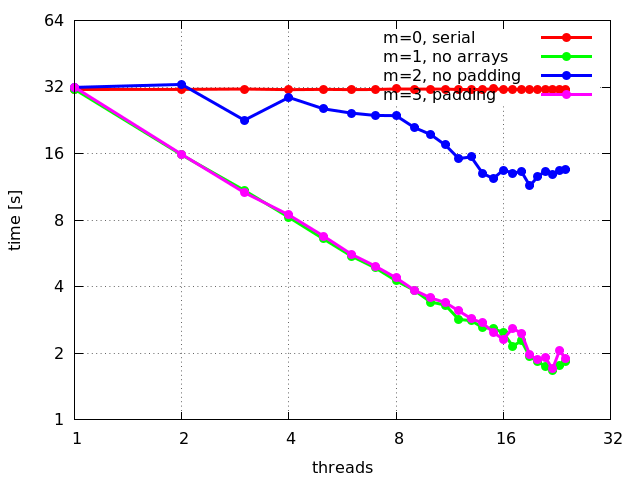
\includegraphics[width=\textwidth]{plots/scaling_euler_O0.png}
    \caption{Scaling behavior on Euler cluster for 4 different implementations. Parameter $-O0$.}
    \label{fig:euler_O0}
  \end{minipage}
  \hfill
  \begin{minipage}[t]{0.45\textwidth}
    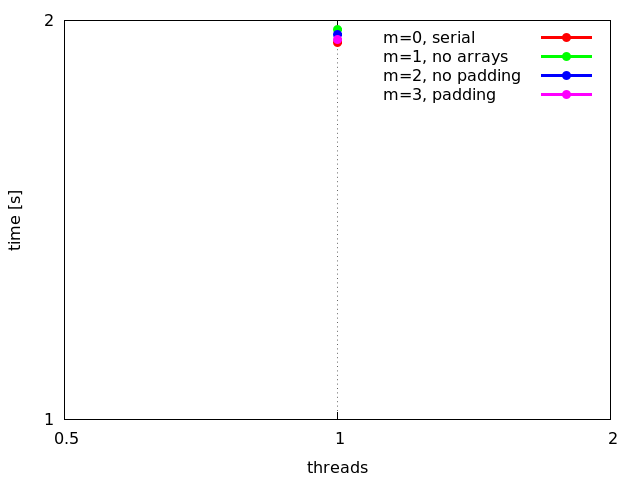
\includegraphics[width=1\textwidth]{plots/scaling_euler_O3.png}
    \caption{Scaling behavior on Euler cluster for 4 different implementations. Parameter $-O3$.}
    \label{fig:euler_O3}
  \end{minipage}
\end{figure}

\item
The work $N$ is equal among all threads $n$ as $N$ tends to infinity. We divide the number of times we draw our random numbers by all threads. We assume that every evaluation of the PRNG takes the same time and therefore every loop iteration as well. This means that the difference of the workload per thread gets negligible for large $N$, even when $N$ is not a multiple of $n$. The maximum load-imbalance is one loop iteration. The code is very close to achieving perfect scaling, but falls off a bit for higher thread numbers. We assume this is because of the overhead of spawning the different processes compared to the relatively small workload of $1e8$. On $24$ threads this leaves a merely $4$ million iterations per thread. Additionally, the spawning of the random number generator and setting the seeds in the implementation where only `omp parallel for reduction` is allowed is done in the OpenMP master, which is serial. The serial fraction will become smaller as our workload $N$ increases, leading to a better scaling behavior. The numerical results we get are the same every time we run it on the serial code and with just one OpenMP thread. However, when running with more than one OpenMP thread, we have slightly different results every time. We assume this is because the order of summation in the reduction is different for different executions, leading to different numerical rounding and therefore also result. 

\end{enumerate}

\section{OpenMP Bug Hunting I}
We have a race condition with the variable \texttt{pos}, as the read access on line $14$ is not together with the increase of the variable on line $17$. A possible scenario with two threads $\mathcal{A}$ and $\mathcal{B}$ demonstrates the issue:
\begin{enumerate}
    \item Thread $\mathcal{A}$ finds a good member $i$ at location 1.
    \item Thread $\mathcal{A}$ assigns 1 to \texttt{good\_members[0]}.
    \item Thread $\mathcal{B}$ finds a good member at location $512$.
    \item Thread $\mathcal{A}$ assigns 512 to \texttt{good\_members[0]}.
    \item Thread $\mathcal{B}$ updates \texttt{pos} to $1$.
    \item Thread $\mathcal{A}$ updates \texttt{pos} to $2$.
\end{enumerate}

One possible solution would be to wrap the read and write of the \texttt{pos} variable in a critical section, like so:

\begin{minted}{cpp}
if(is_good(i){ 
    #pragma omp critical
    {
        good_members[pos] = i;
        pos++;
    }
}
\end{minted}


\section{OpenMP Bug Hunting II}
\begin{enumerate}[a)]
\setcounter{enumi}{0}
\item
Analyzing the code in Question $3a$ we find the following bugs:
\begin{enumerate}[1]
    \item The arrays \texttt{a}, \texttt{b}, \texttt{c}\ and \texttt{z} are all neither declared nor initialized. This can be fixed by declaring and initializing the four arrays.
    \item Every thread will execute the for-loop on line $13$ completely, which means that we'll have nested parallelism (I assume this is not intended). The nested parallelism can be removed by removing the \texttt{parallel} on line $15$.
    \item There is a data race for the arrays \texttt{b} and \texttt{c} because of the \texttt{nowait} on line $15$ and the access in line $23$. Removing the \texttt{nowait} clause will fix this issue.
\end{enumerate}
\item
Analyzing the code in Question $3a$ we propose the following improvements: the \texttt{\#pragma omp parallel} and \texttt{\#pragma omp for} can be grouped into one OpenMP statement, namely \texttt{\#pragma omp parallel for}. The best improvement is achieved when grouping all four OpenMP statements, thereby removing the nested parallelism. This can be done as each loop consists of only one statement. The resulting code would then read as follows:

\begin{minted}{cpp}
void work(int i, int j);

void nesting(int n){
    int i, j;
    #pragma omp parallel for collapse(2)
    for (i=0; i<n; i++){
        for(j=0; j<n; j++){
            work(i, j);
        }
    }
}
\end{minted}

\end{enumerate}

\bigskip
%----------------------------------------------------------------------------------------
%	REFERENCE LIST
%----------------------------------------------------------------------------------------

\printbibliography

%----------------------------------------------------------------------------------------

\end{document}

